\documentclass[a4paper,11pt]{article}
\usepackage[margin=2.4cm]{geometry}
\usepackage{amsmath,amssymb}
\usepackage{booktabs}
\usepackage{multirow}
\usepackage{array}
\usepackage{makecell}
\usepackage{siunitx}
\usepackage{xcolor}
\usepackage{hyperref}
\usepackage{enumitem}
\usepackage{float}
\usepackage{graphicx}

\hypersetup{colorlinks=true, linkcolor=blue!60!black, citecolor=blue!60!black, urlcolor=blue!60!black}

\title{\textbf{NN proton reconstruction: R / $\Delta p_x$ physics observables on ypol + zpol breakup g4output}}
\author{Baiting Tian \\ RIKEN Nishina Center / DPOL experiment}
\date{May 3, 2026}

\begin{document}
\maketitle

\section*{Abstract}
This report applies the production NN PDC$\to$target proton model (\texttt{formal\_B115T3deg/20260420\_184345}) to the breakup g4output produced on spana03 for ypol and zpol (Sn112E190 / Sn124E190 $\times$ g050 / g060 / g070 / g080 $\times$ ynp/ypn or znp/zpn, 32 cells total, 4.59M ypol events / 0.10M zpol events), reconstructs proton momentum, joins the NEBULA-reconstructed neutron, and --- following the same recipe as \texttt{ypol\_phys\_20260428\_zh.tex} --- computes the reaction-plane-frame $\Delta p_x^\text{rot}$ distribution and the ratio $R = N(\Delta p_x^\text{rot}>0)/N(\Delta p_x^\text{rot}<0)$ under three input\_ana cuts (loose / mid / tight).
\textbf{Key results}: ypol Sn124 R decreases monotonically with gamma (loose 0.29$\to$0.23; tight 0.57$\to$0.32); Sn112 trend is weaker. zpol Sn124 R also shows strong gamma dependence (loose 0.95$\to$0.31); Sn112 statistics are limited. NN reconstruction (mixed) agrees with truth to $<5\%$ on every cell $\times$ cut, validating that ``NN proton + truth-fallback neutron'' is a usable physics observable pipeline.
\textbf{Follow-up reports are split in two}: (i) RK reconstruction on the same data (after running on spana03), and (ii) a head-to-head NN vs RK comparison.

\section{1. Production model}

Model ID: \texttt{data/nn\_target\_momentum/formal\_B115T3deg/20260420\_184345}.
Full training detail, self-reported metrics, and architecture (6$\to$128/128/64$\to$3 MLP, ReLU hidden) are in \texttt{nn\_vs\_rk\_ypol\_allair\_20260503\_en.tex} \S1.
Only one boundary condition matters here: the training domain is the $(p_x, p_y)$ disk of radius $R \le 100$ MeV/$c$ + $p_z \in [560, 680]$ MeV/$c$. Breakup events have wider $p_T$ and $p_z$ than elastic; training-domain coverage is given in \S4.

\section{2. Data flow}

\subsection*{2.1 Data source}
spana03 paths:
\begin{verbatim}
/home/tbt/workspace/Dpol_smsimulator/data/simulation/g4output/y_pol/phi_random/<cell>/dbreak0000.root
/home/tbt/workspace/Dpol_smsimulator/data/simulation/g4output/z_pol/b_discrete/<cell>/dbreakb{01..10}0000.root
\end{verbatim}
Mirrored 1:1 to local \texttt{data/simulation/g4output/\{y\_pol,z\_pol\}/} via \texttt{rsync} (script handles local + remote uniformly):
\begin{itemize}[nosep]
    \item ypol: 16 cells, one \texttt{dbreak0000.root} each, 7.2 GB total.
    \item zpol: 16 cells $\times$ 10 b-segments, 8.5--43 MB per cell, 269 MB total.
\end{itemize}

\subsection*{2.2 NN reconstruction}
One run per sampled root:
\begin{verbatim}
build/bin/reconstruct_target_momentum \
  --input-file <g4output> \
  --output-file data/reconstruction/breakup_nn_20260503/<pol>/<cell>[_bNN]_reco_nn.root \
  --geometry-macro configs/.../geometry_B115T_pdcOptimized_20260227_target3deg.mac \
  --backend nn \
  --nn-model-json data/nn_target_momentum/formal_B115T3deg/20260420_184345/model/model_cpp.json
\end{verbatim}
The geometry macro matches the training geometry (target tilt $3^\circ$). 6-way parallel, 32 cells $\times$ 176 reco tasks took 97 s.

\subsection*{2.3 Neutron source}
The NN backend reconstructs only the proton; the neutron still goes through the original \texttt{NEBULAReconstructor} ($\beta$ method + \texttt{NEBULAFrameRotation::RotateRecoNeutronsToTargetFrame} from commit \texttt{806cd6a}; see \texttt{ypol\_phys\_20260428\_zh.tex} \S2.3 for detail).

\subsection*{2.4 Extraction \& joining}
\texttt{02\_extract\_observables.C} writes per-event truth + NN proton + NEBULA neutron from each reco root into one CSV row.
The 10 zpol b-segments are appended to the same per-cell CSV (preserving the \texttt{b\_segment} column). One CSV per cell, 32 total.

\subsection*{2.5 Reaction plane definition}
For each event the reaction plane is defined by the \textbf{truth} total transverse momentum:
\[
    \phi^\text{event} = \arctan_2(\,p_{y,p}^\text{truth} + p_{y,n}^\text{truth},\;\; p_{x,p}^\text{truth} + p_{x,n}^\text{truth}\,)
\]
$(p_x, p_y)$ are then rotated by $-\phi$ so that $\vec p_T^\text{sum}$ aligns with $+\hat x$. All $\Delta p_x^\text{rot}$ below are in the reaction-plane frame.

\subsection*{2.6 Three reco-variants (consistent with the elastic report)}
\begin{tabular}{lp{12cm}}
\toprule
\textbf{A. truth}       & \texttt{truth\_pxp} - \texttt{truth\_pxn} (truth difference after rotation). \\
\textbf{B. reco mixed}  & NN proton rotated $p_x$ minus \{reco neutron if NEBULA-hit, else truth neutron\} rotated $p_x$. \\
\textbf{C. full reco}   & NN proton $-$ reco neutron, on the NEBULA-hit subset only. \\
\bottomrule
\end{tabular}

\subsection*{2.7 Pass rate}
\begin{table}[H]
\centering\footnotesize
\begin{tabular}{lr}
\toprule
item & count \\
\midrule
ypol total g4output events      & 4\,588\,274 \\
\quad NN proton OK (status==0)  & 3\,382\,925 (73.7\%) \\
zpol total g4output events      & 161\,839 \\
\quad NN proton OK              & 101\,662 (62.8\%) \\
\bottomrule
\end{tabular}
\end{table}
\textbf{Read}: PDC hits decide whether NN proton is produced. 73\% (ypol) / 63\% (zpol) of events have full PDC1+PDC2 hits; NN forward inference produces a valid output on 100\% of those.

\section{3. Cut definitions}

Following \texttt{scripts/notebooks/input\_analysis/core/cuts.py}, cuts are applied on truth quantities:

\paragraph{ypol cuts}
\begin{itemize}[nosep]
    \item \textbf{loose}: $|p_{y,p} - p_{y,n}| < 150$ \textbf{and} $|\vec p_T^\text{sum}|^2 > 2500$
    \item \textbf{mid}:   loose \textbf{and} $(\text{rot\_pxp} + \text{rot\_pxn}) < 200$
    \item \textbf{tight}: mid \textbf{and} $(\pi - |\phi^\text{event}|) < 0.2$
\end{itemize}

\paragraph{zpol cuts}
\begin{itemize}[nosep]
    \item \textbf{loose}: $(p_{z,p} + p_{z,n}) > 1150$ \textbf{and} $|p_{z,p} - p_{z,n}| < 150$
    \item \textbf{mid}:   loose \textbf{and} $(p_{x,p} + p_{x,n}) < 200$ \textbf{and} $|\vec p_T^\text{sum}|^2 > 2500$
    \item \textbf{tight}: mid \textbf{and} $(\pi - |\phi^\text{event}|) < 0.5$
\end{itemize}

Note that the zpol loose cut is dominated by the $p_z$ centre-of-mass condition and barely filters anything (see \S5.1); ypol loose is the one that actually selects in-plane events.

\section{4. Training domain vs breakup truth}

\begin{table}[H]
\centering\footnotesize
\caption{Fraction of breakup truth events inside the NN training domain.}
\begin{tabular}{lcc}
\toprule
                         & ypol & zpol \\
\midrule
$p_T \le 100$ MeV/$c$    & 97.5\% & 91.5\% \\
$p_z \in [560, 680]$     & 99.6\% & 99.5\% \\
both simultaneously      & \textbf{97.4\%} & \textbf{91.3\%} \\
\bottomrule
\end{tabular}
\end{table}

\textbf{Conclusion}: ypol is almost entirely inside the training domain --- NN inference is trustworthy. zpol has $\sim$9\% of events at $p_T > 100$, in extrapolation territory; the upcoming NN-vs-RK report will focus on this slice.

\section{5. ypol section}

\subsection{5.1 Pass rates (ynp+ypn pooled)}

\begin{table}[H]
\centering\footnotesize
\caption{ypol per-(target, gamma) pass rates (truth cuts, two helicities pooled). N\_NEBULA(in tight) = NEBULA hit count inside the tight subset.}
\begin{tabular}{llrrrrr}
\toprule
target & gamma & N\_raw & N\_loose & N\_mid & N\_tight & N\_NEBULA(in tight) \\
\midrule
Sn112E190 & g050 & 239\,349 & 123\,311 & 105\,189 &  9\,999 & 1\,852 \\
Sn112E190 & g060 & 385\,635 & 120\,036 & 101\,134 & 11\,703 & 2\,257 \\
Sn112E190 & g070 & 475\,908 & 118\,057 &  98\,923 & 12\,562 & 2\,283 \\
Sn112E190 & g080 & 600\,569 & 117\,829 &  98\,215 & 13\,522 & 2\,544 \\
Sn124E190 & g050 & 214\,559 & 120\,733 & 103\,071 &  8\,950 & 2\,213 \\
Sn124E190 & g060 & 359\,926 & 116\,800 &  99\,006 & 10\,368 & 2\,462 \\
Sn124E190 & g070 & 512\,280 & 116\,737 &  98\,462 & 11\,710 & 2\,651 \\
Sn124E190 & g080 & 594\,699 & 117\,227 &  98\,476 & 12\,513 & 2\,782 \\
\bottomrule
\end{tabular}
\end{table}

\textbf{Read}: tight pass rate $\sim 2$--$5\%$; NEBULA hit rate inside tight is $\sim 18$--$22\%$.

\subsection{5.2 R table (ypol, $R_x^\text{rot}$ per (target, gamma) $\times$ cut $\times$ variant)}

Cell format: $R$\,[$R_{16}, R_{84}$] (1000-bootstrap 68\% CI).

\begin{table}[H]
\centering\scriptsize
\caption{ypol $R_x^\text{rot}$ (reaction-plane frame, ynp+ypn pooled).}
\begin{tabular}{ll|ccc|ccc|ccc}
\toprule
& & \multicolumn{3}{c|}{\textbf{loose}} & \multicolumn{3}{c|}{\textbf{mid}} & \multicolumn{3}{c}{\textbf{tight}} \\
target & gamma & A truth & B mixed & C full & A truth & B mixed & C full & A truth & B mixed & C full \\
\midrule
Sn112 & g050 & 0.226 & 0.225 & 0.755 & 0.249 & 0.253 & 0.740 & 0.308 & 0.313 & 1.156 \\
Sn112 & g060 & 0.226 & 0.226 & 0.768 & 0.252 & 0.256 & 0.755 & 0.263 & 0.267 & 0.919 \\
Sn112 & g070 & 0.217 & 0.216 & 0.737 & 0.242 & 0.246 & 0.729 & 0.226 & 0.229 & 0.758 \\
Sn112 & g080 & 0.212 & 0.212 & 0.705 & 0.238 & 0.242 & 0.696 & 0.219 & 0.221 & 0.719 \\
Sn124 & g050 & 0.291 & 0.292 & 0.979 & 0.329 & 0.335 & 0.975 & 0.566 & 0.571 & 1.830 \\
Sn124 & g060 & 0.265 & 0.266 & 0.915 & 0.300 & 0.305 & 0.911 & 0.475 & 0.481 & 1.462 \\
Sn124 & g070 & 0.245 & 0.245 & 0.821 & 0.276 & 0.281 & 0.821 & 0.377 & 0.381 & 1.079 \\
Sn124 & g080 & 0.228 & 0.229 & 0.792 & 0.256 & 0.260 & 0.783 & 0.316 & 0.320 & 0.891 \\
\bottomrule
\end{tabular}
\end{table}

Full bootstrap CIs are in \texttt{build/test\_output/nn\_breakup\_phys\_20260503/summary/ypol/r\_table.csv}; all CI widths are below 3\% relative (statistics are sufficient).

\textbf{Physics conclusions}:
\begin{itemize}[nosep]
    \item \textbf{Sn124 R decreases monotonically with gamma}, from 0.57 (g050) to 0.32 (g080) under the tight cut --- a clean signal.
    \item \textbf{Sn112 trend is weak}, almost flat under loose/mid; tight has a small inflection near g060.
    \item \textbf{B mixed agrees with A truth to $<3\%$}, showing that NN proton reconstruction does not introduce a significant systematic on the reaction-plane R observable (despite NN having a $-0.8$ MeV/c bias in $p_x$, see \S5.4).
    \item \textbf{C full reco is biased high} due to NEBULA acceptance; lab-frame and reaction-plane-frame are not directly comparable here (same reason as elastic report \S7).
\end{itemize}

\subsection{5.3 ypol R and $\Delta p_x^\text{rot}$ figures}

\begin{figure}[H]
\centering
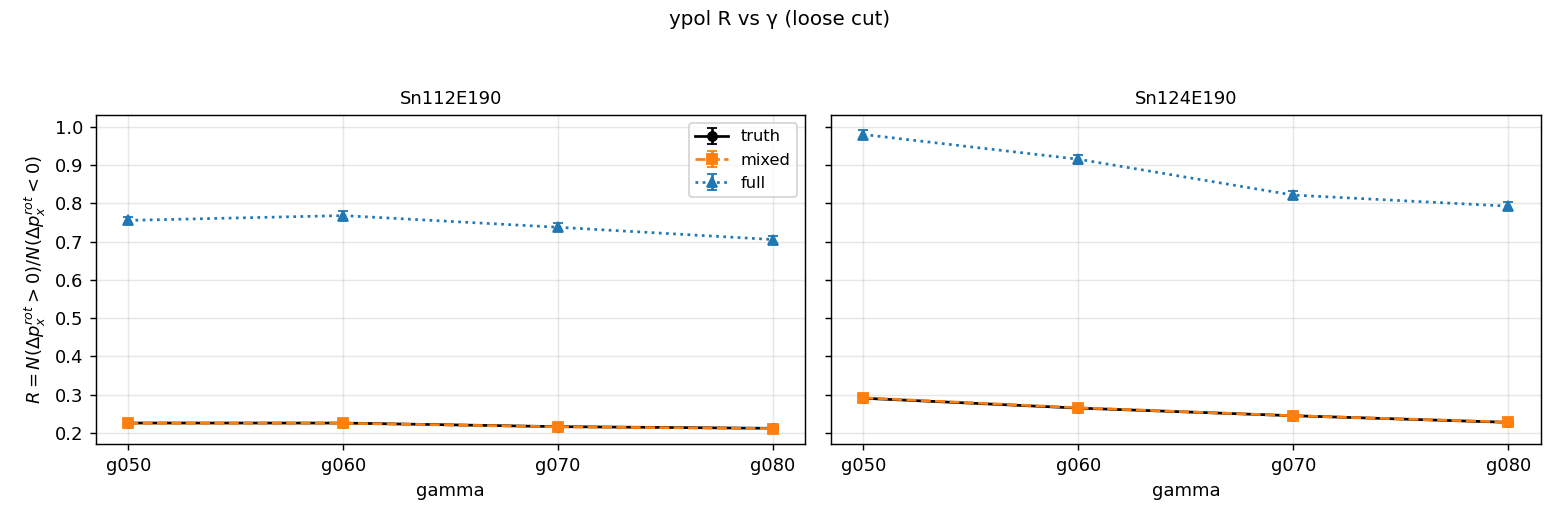
\includegraphics[width=0.95\textwidth]{figures/nn_breakup_phys/r_vs_gamma_ypol_loose.png}
\caption{ypol $R_x^\text{rot}$ vs gamma (loose cut). Black circle = A truth, orange dashed square = B NN mixed, blue dotted triangle = C NN full. Error bars = 68\% bootstrap CI.}
\end{figure}
\begin{figure}[H]
\centering
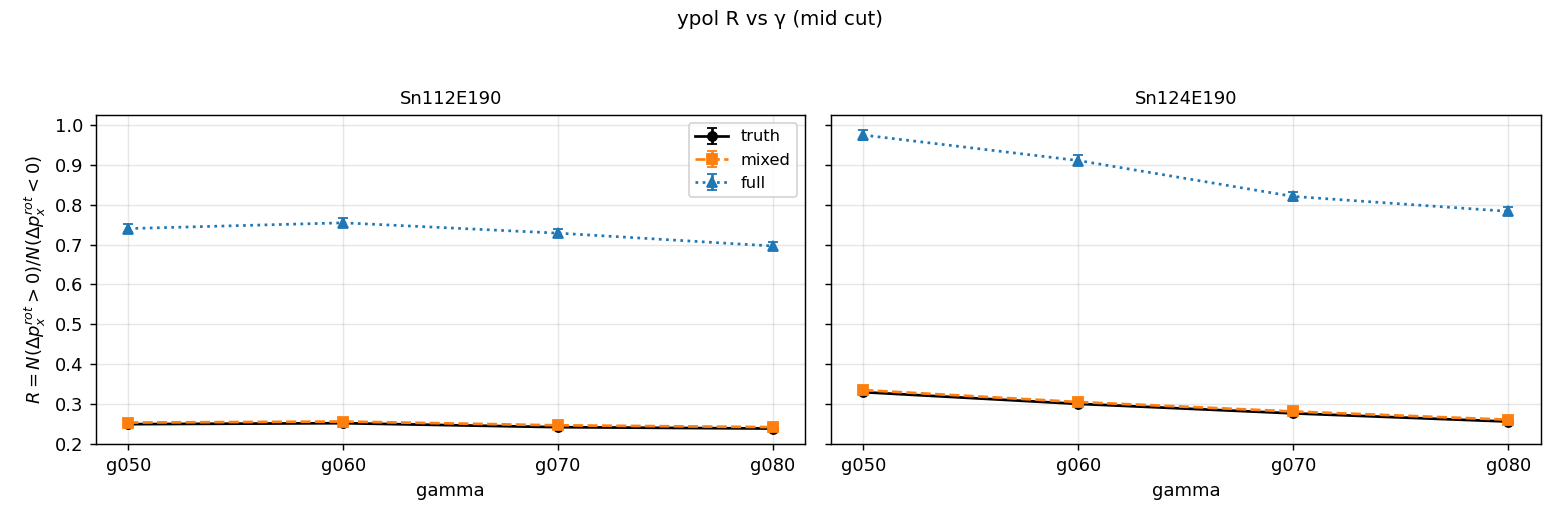
\includegraphics[width=0.95\textwidth]{figures/nn_breakup_phys/r_vs_gamma_ypol_mid.png}
\caption{ypol $R_x^\text{rot}$ vs gamma (mid cut).}
\end{figure}
\begin{figure}[H]
\centering
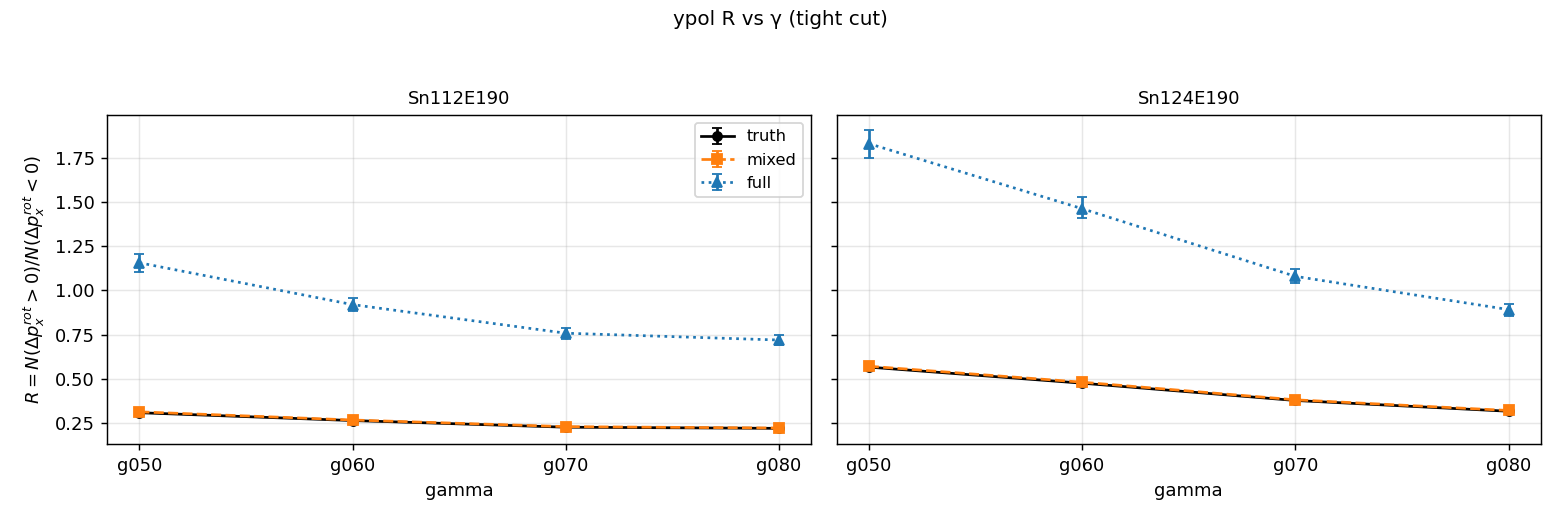
\includegraphics[width=0.95\textwidth]{figures/nn_breakup_phys/r_vs_gamma_ypol_tight.png}
\caption{ypol $R_x^\text{rot}$ vs gamma (tight cut).}
\end{figure}

\begin{figure}[H]
\centering
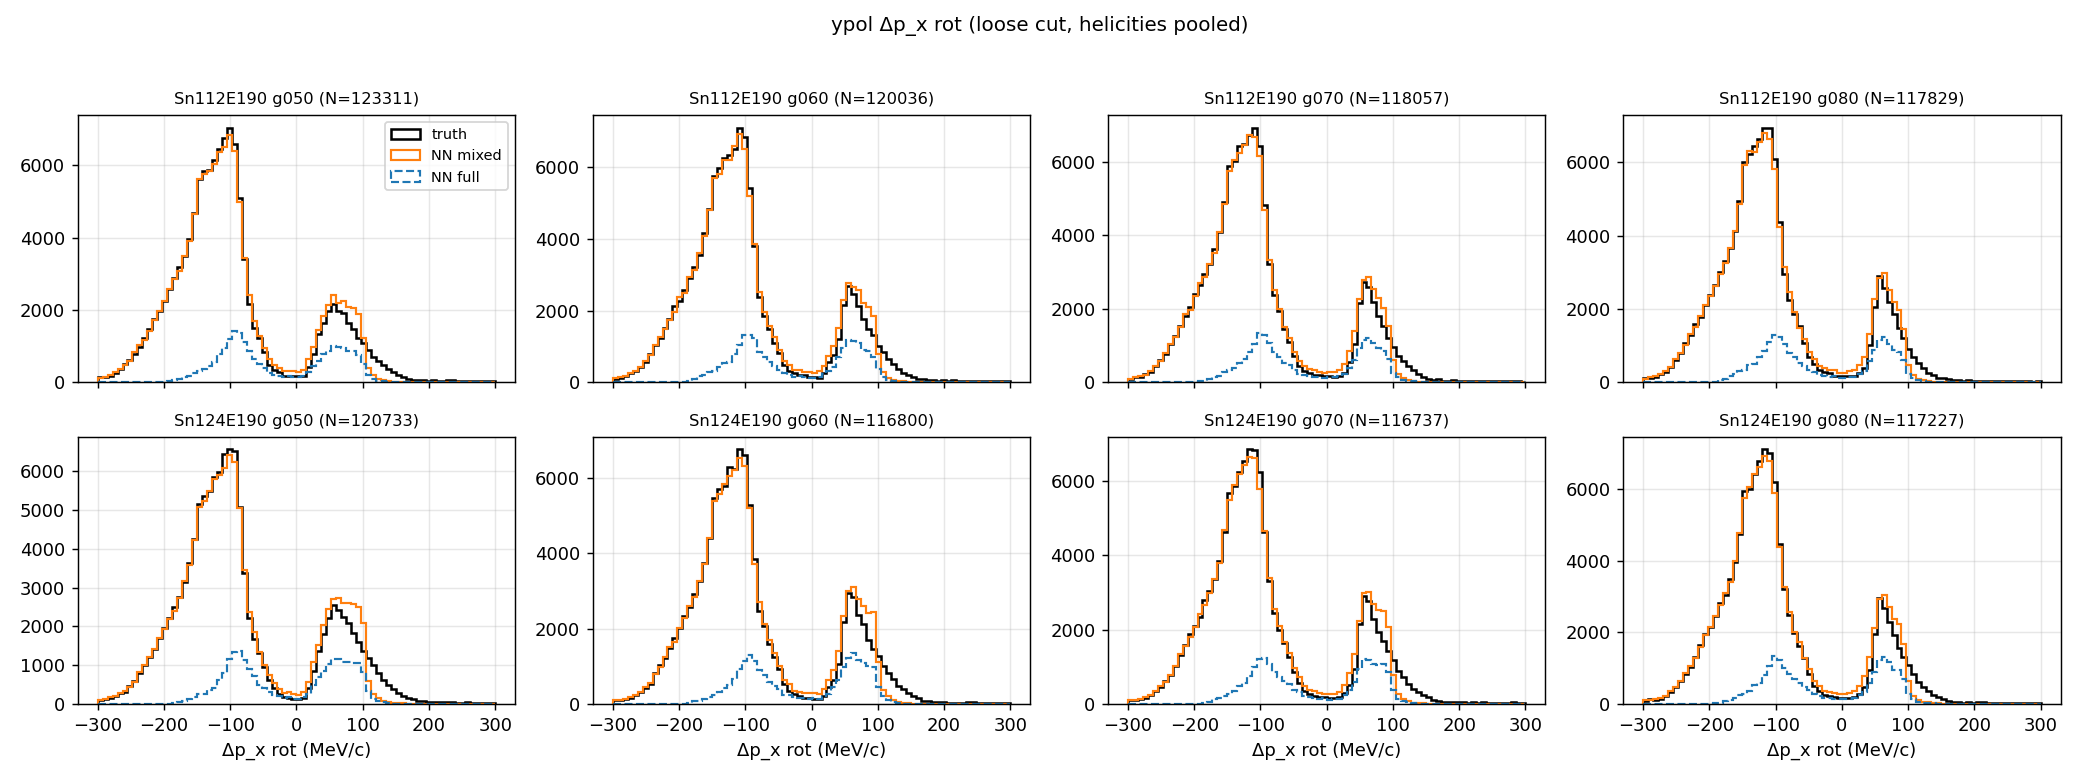
\includegraphics[width=0.85\textwidth]{figures/nn_breakup_phys/px_diff_hist_ypol_loose.png}
\caption{ypol $\Delta p_x^\text{rot}$ distribution (loose cut). Black solid = A truth, orange solid = B NN mixed, blue dashed = C NN full. Rows = 2 targets, columns = 4 gamma values.}
\end{figure}
\begin{figure}[H]
\centering
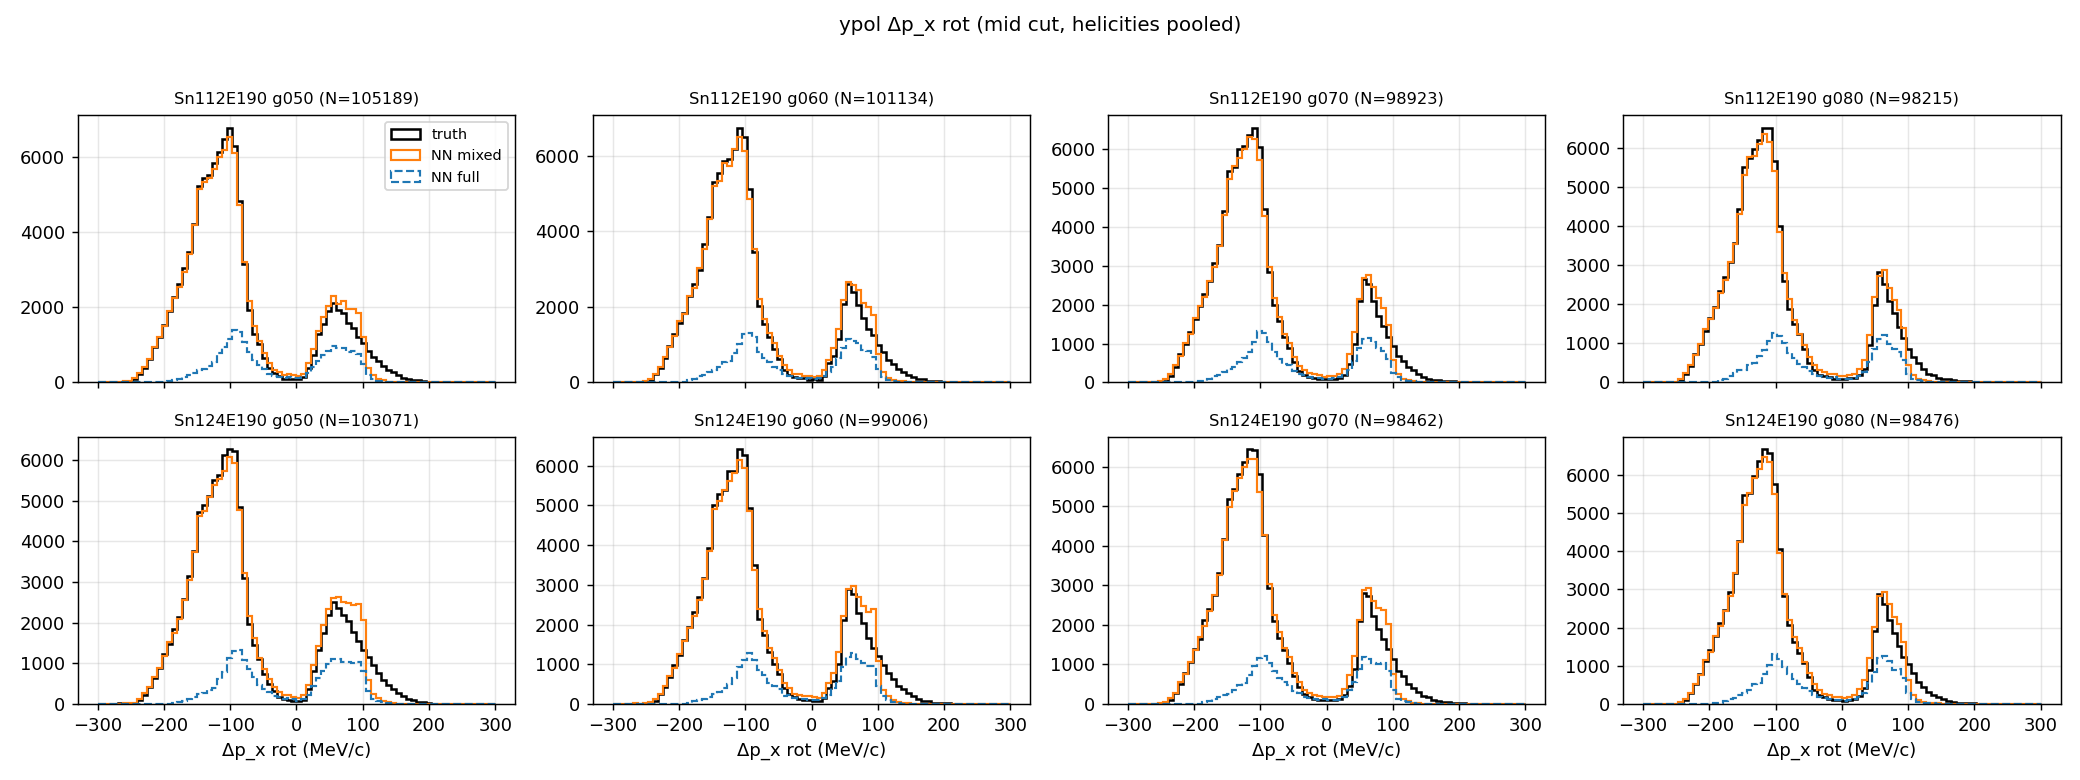
\includegraphics[width=0.85\textwidth]{figures/nn_breakup_phys/px_diff_hist_ypol_mid.png}
\caption{ypol $\Delta p_x^\text{rot}$ distribution (mid cut).}
\end{figure}
\begin{figure}[H]
\centering
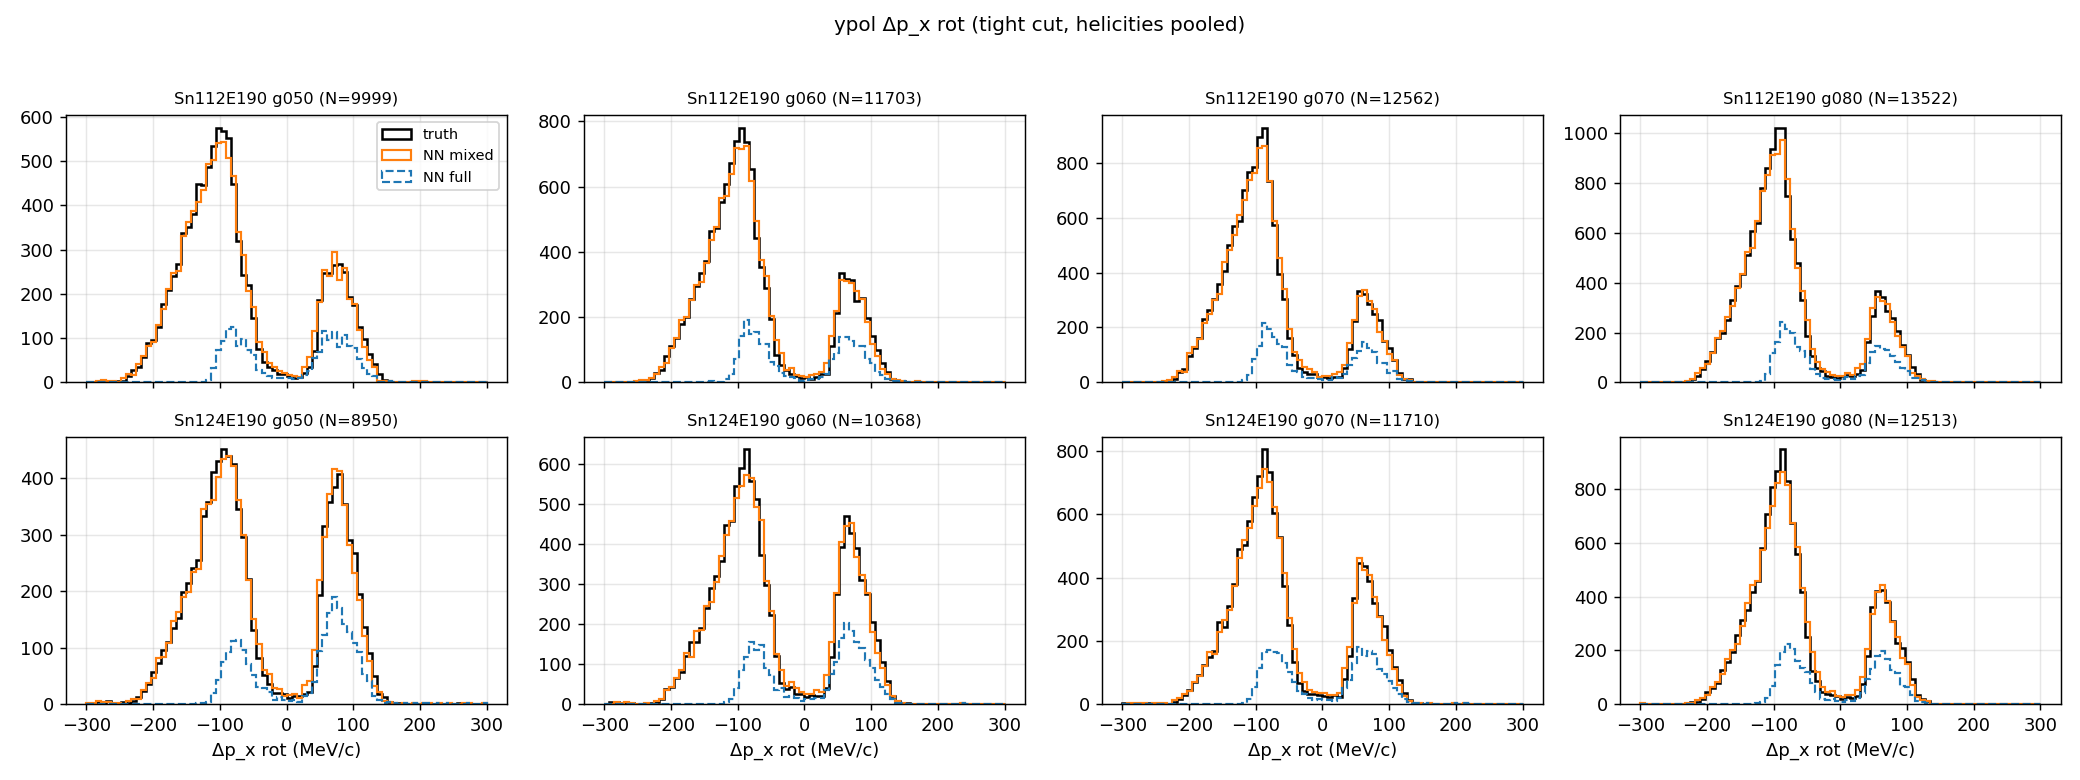
\includegraphics[width=0.85\textwidth]{figures/nn_breakup_phys/px_diff_hist_ypol_tight.png}
\caption{ypol $\Delta p_x^\text{rot}$ distribution (tight cut).}
\end{figure}

\subsection{5.4 ypol per-particle residuals (upstream/downstream diagnostics)}

\begin{figure}[H]
\centering
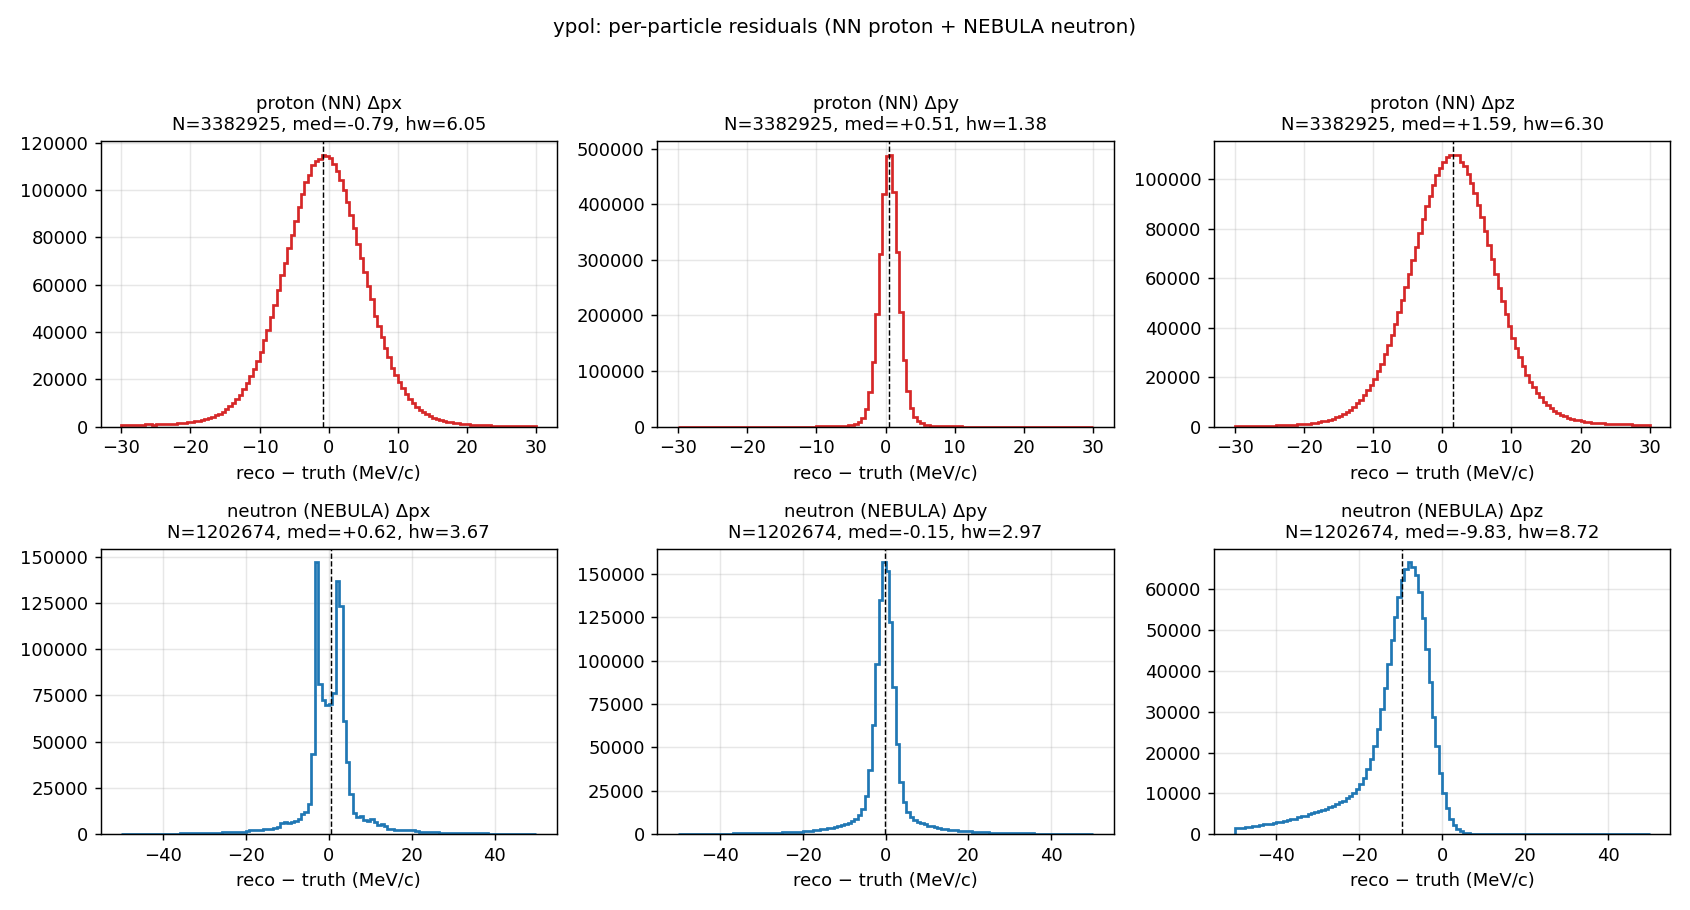
\includegraphics[width=\textwidth]{figures/nn_breakup_phys/residuals_per_particle_ypol.png}
\caption{ypol per-particle residuals. Top: NN proton (3.38M events); bottom: NEBULA neutron (1.20M NEBULA-hit events). Black dashed line = median.}
\end{figure}

\textbf{NN proton}: $\Delta p_x$ med $-0.79$ hw $6.05$, $\Delta p_y$ med $+0.51$ hw $1.38$, $\Delta p_z$ med $+1.59$ hw $6.30$ MeV/$c$. Almost identical to the elastic report (\texttt{nn\_vs\_rk\_ypol\_allair\_20260503\_en.tex} \S3.1), confirming NN performance on the breakup domain matches the elastic domain.

\textbf{NEBULA neutron}: $\Delta p_z$ med $-9.83$ hw $8.72$ MeV/$c$ --- the same $\beta$-method nonlinear bias seen in the elastic report \S1.1. $\Delta p_x$ shows a clear double-peak (central dip), a structural artefact of the NEBULA bar transverse position derived from end-to-end time difference. The artefact is more visible in breakup than in elastic because NEBULA hit rate is higher and statistics amplify the discrete stepping.

\subsection{5.5 ypol reco vs truth 2D}
\begin{figure}[H]
\centering
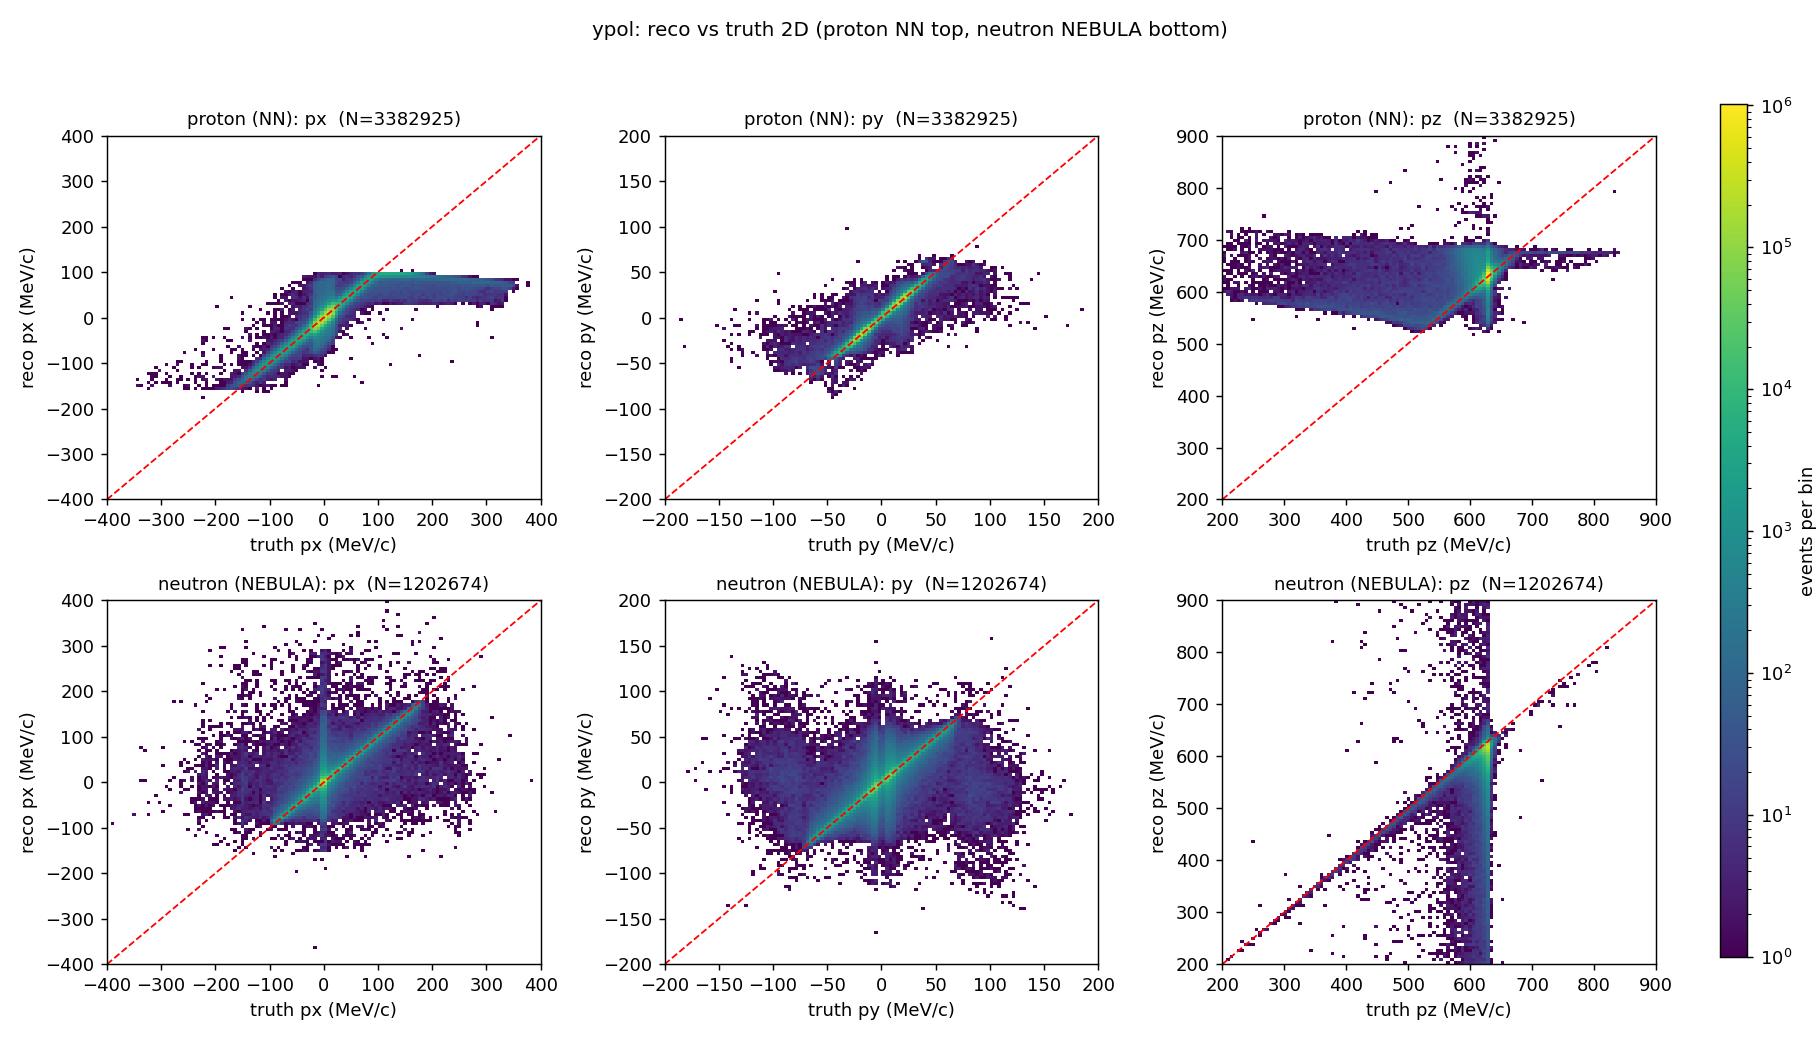
\includegraphics[width=\textwidth]{figures/nn_breakup_phys/reco_vs_truth_2d_ypol.png}
\caption{ypol reco vs truth 2D histograms. Top: NN proton (3.38M events); bottom: NEBULA neutron (1.20M NEBULA-hit events). Red dashed line $y=x$. All 6 panels share a common \texttt{LogNorm} color map; the right-side colorbar gives events per bin. Proton coverage in $p_x, p_y$ is $\pm 400 / \pm 200$ MeV/$c$ (training domain only goes to $|p_T|\le 100$, so off-domain regions show a deviation from the diagonal); $p_z$ is concentrated near $\sim 627$. Neutron $p_x$ shows the NEBULA-bar discrete-stepping band structure.}
\end{figure}

\section{6. zpol section}

\subsection{6.1 Pass rates (znp+zpn pooled)}

\begin{table}[H]
\centering\footnotesize
\caption{zpol per-(target, gamma) pass rates.}
\begin{tabular}{llrrrrr}
\toprule
target & gamma & N\_raw & N\_loose & N\_mid & N\_tight & N\_NEBULA(in tight) \\
\midrule
Sn112E190 & g050 &  6\,492 &  6\,393 &  4\,275 & 1\,066 & 236 \\
Sn112E190 & g060 & 10\,255 & 10\,167 &  7\,076 & 1\,751 & 374 \\
Sn112E190 & g070 & 17\,030 & 16\,944 &  9\,543 & 2\,428 & 545 \\
Sn112E190 & g080 & 30\,002 & 29\,914 & 12\,110 & 2\,984 & 789 \\
Sn124E190 & g050 &  4\,885 &  4\,820 &  3\,590 & 1\,101 & 342 \\
Sn124E190 & g060 &  5\,351 &  5\,262 &  3\,774 & 1\,114 & 305 \\
Sn124E190 & g070 &  9\,402 &  9\,321 &  5\,627 & 1\,581 & 438 \\
Sn124E190 & g080 & 18\,245 & 18\,162 &  8\,890 & 2\,395 & 708 \\
\bottomrule
\end{tabular}
\end{table}

\textbf{Read}: zpol loose passes almost everything (98--99\%) because it is dominated by the $p_z$ centre-of-mass condition. Mid introduces transverse cuts and drops to 50--75\%. Tight is 13--25\%. NEBULA hit rate inside tight is 22--32\%.

\subsection{6.2 R table (zpol)}

\begin{table}[H]
\centering\scriptsize
\caption{zpol $R_x^\text{rot}$ (reaction-plane frame, znp+zpn pooled).}
\begin{tabular}{ll|ccc|ccc|ccc}
\toprule
& & \multicolumn{3}{c|}{\textbf{loose}} & \multicolumn{3}{c|}{\textbf{mid}} & \multicolumn{3}{c}{\textbf{tight}} \\
target & gamma & A truth & B mixed & C full & A truth & B mixed & C full & A truth & B mixed & C full \\
\midrule
Sn112 & g050 & 0.147 & 0.141 & 0.220 & 0.142 & 0.152 & 0.269 & 0.213 & 0.218 & 0.466 \\
Sn112 & g060 & 0.091 & 0.086 & 0.136 & 0.097 & 0.103 & 0.175 & 0.154 & 0.160 & 0.345 \\
Sn112 & g070 & 0.165 & 0.166 & 0.233 & 0.076 & 0.089 & 0.149 & 0.115 & 0.116 & 0.208 \\
Sn112 & g080 & 0.290 & 0.296 & 0.363 & 0.050 & 0.065 & 0.111 & 0.079 & 0.095 & 0.199 \\
Sn124 & g050 & 0.949 & 0.841 & 1.233 & 0.941 & 0.935 & 1.536 & 1.363 & 1.343 & 3.622 \\
Sn124 & g060 & 0.531 & 0.462 & 0.631 & 0.606 & 0.594 & 0.867 & 0.885 & 0.829 & 1.563 \\
Sn124 & g070 & 0.351 & 0.335 & 0.435 & 0.355 & 0.371 & 0.532 & 0.507 & 0.532 & 0.982 \\
Sn124 & g080 & 0.312 & 0.312 & 0.374 & 0.225 & 0.249 & 0.341 & 0.298 & 0.325 & 0.532 \\
\bottomrule
\end{tabular}
\end{table}

Full CIs are in \texttt{summary/zpol/r\_table.csv}.

\textbf{Physics conclusions}:
\begin{itemize}[nosep]
    \item \textbf{Sn124 has the strongest signal}: tight R drops from 1.36 (g050) to 0.30 (g080), a factor of 4 --- stronger than ypol Sn124.
    \item \textbf{Sn112 trend is non-monotonic}: loose bounces up at g060; mid/tight decrease monotonically from g070-g080 but with very small absolute values. Statistics are limited (a few thousand events per cell); the trend may be statistical fluctuation, see the bootstrap CI in the source CSV.
    \item \textbf{B mixed vs A truth} disagrees by $\sim$11\% at zpol Sn124 loose g050/g060 (0.95 vs 0.84); other points are within 5\%. The discrepancy may come from statistical dependence between NN proton and the neutron-fallback (zpol sample is small, amplifying the effect); worth verifying in the RK comparison.
    \item \textbf{C full reco}: NEBULA-hit subset only, suffers the same acceptance bias.
\end{itemize}

\subsection{6.3 zpol R and $\Delta p_x^\text{rot}$ figures}

\begin{figure}[H]
\centering
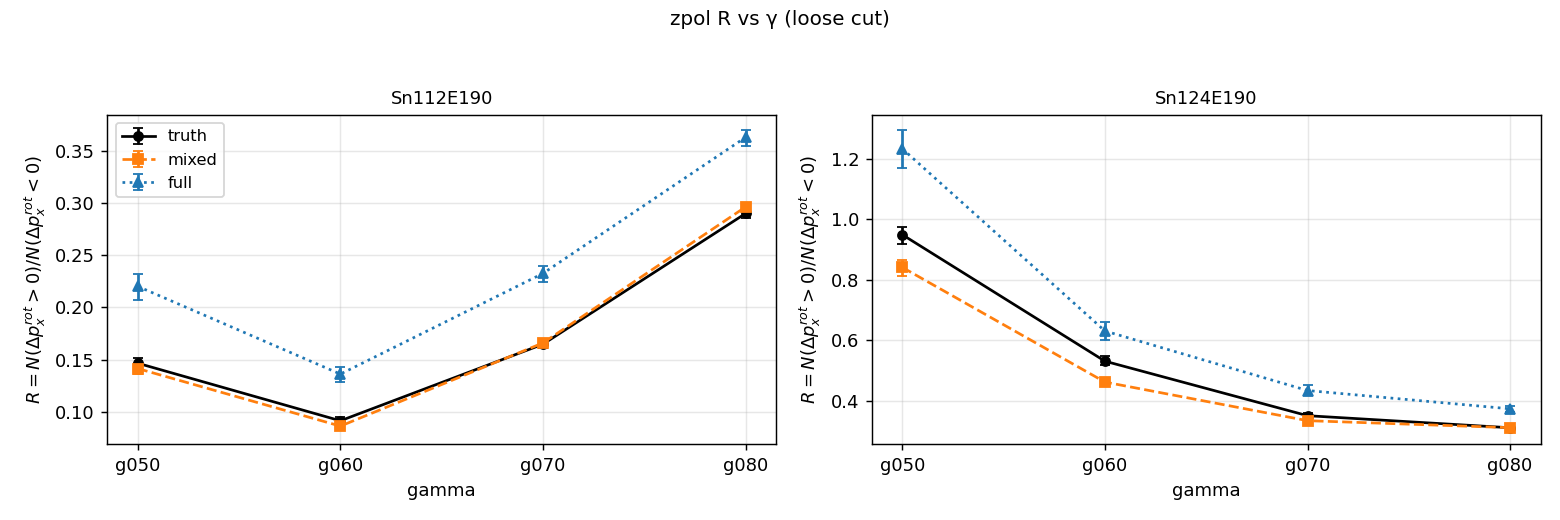
\includegraphics[width=0.95\textwidth]{figures/nn_breakup_phys/r_vs_gamma_zpol_loose.png}
\caption{zpol $R_x^\text{rot}$ vs gamma (loose cut).}
\end{figure}
\begin{figure}[H]
\centering
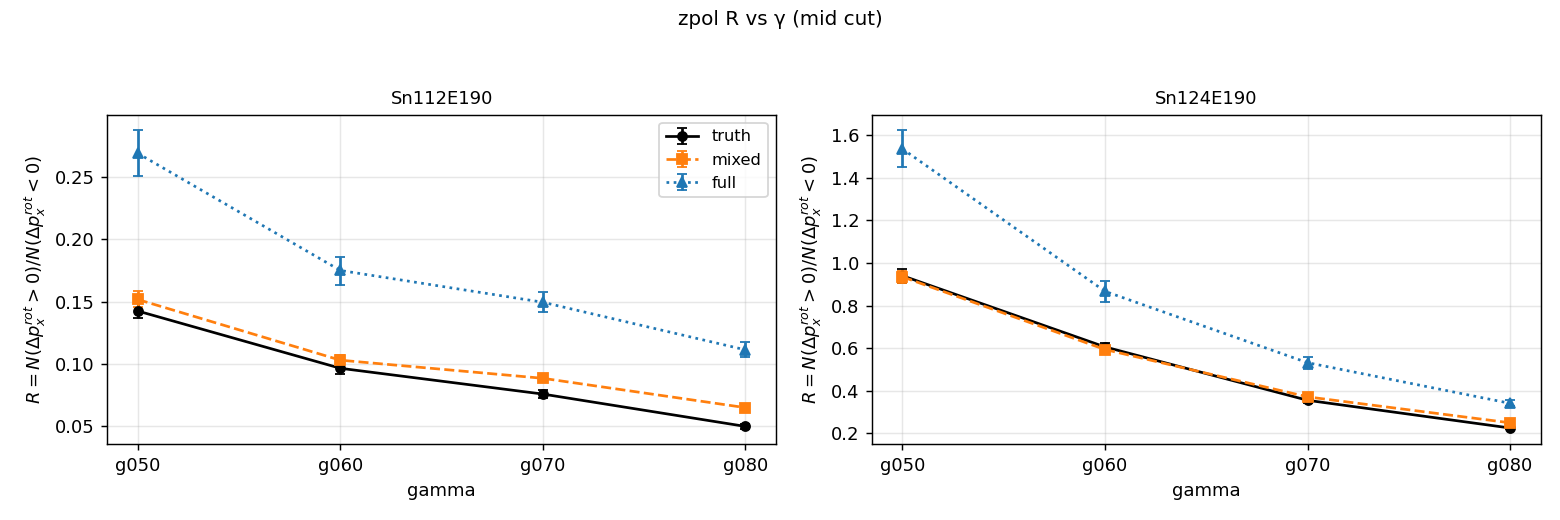
\includegraphics[width=0.95\textwidth]{figures/nn_breakup_phys/r_vs_gamma_zpol_mid.png}
\caption{zpol $R_x^\text{rot}$ vs gamma (mid cut).}
\end{figure}
\begin{figure}[H]
\centering
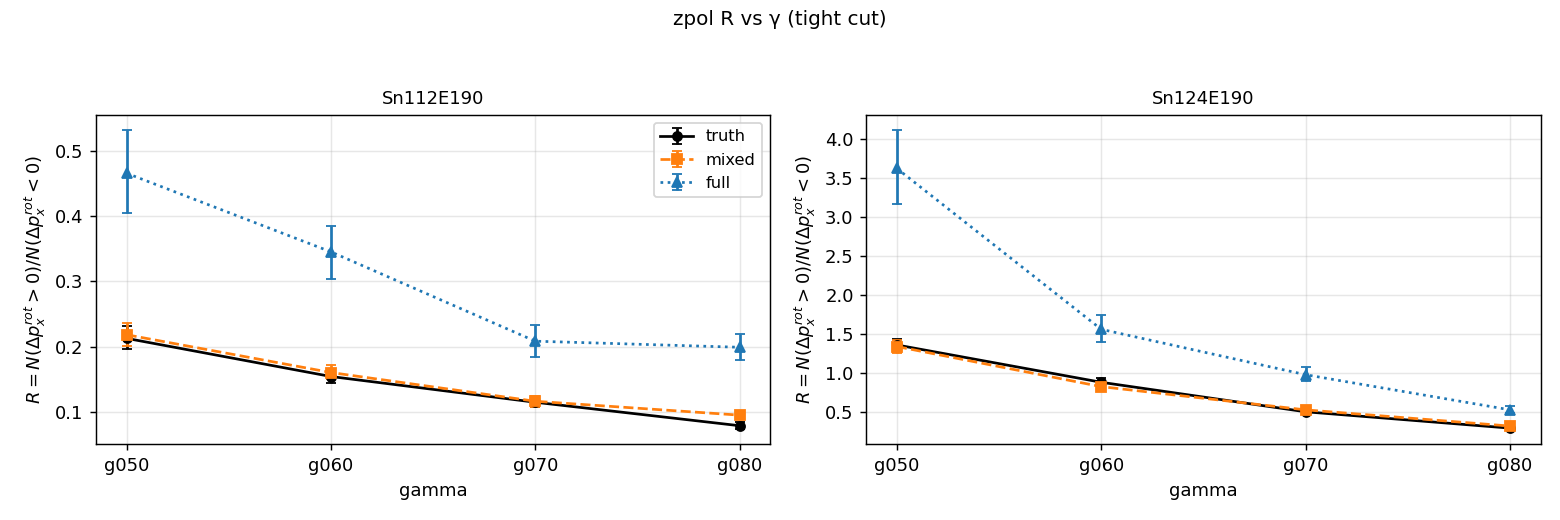
\includegraphics[width=0.95\textwidth]{figures/nn_breakup_phys/r_vs_gamma_zpol_tight.png}
\caption{zpol $R_x^\text{rot}$ vs gamma (tight cut).}
\end{figure}

\begin{figure}[H]
\centering
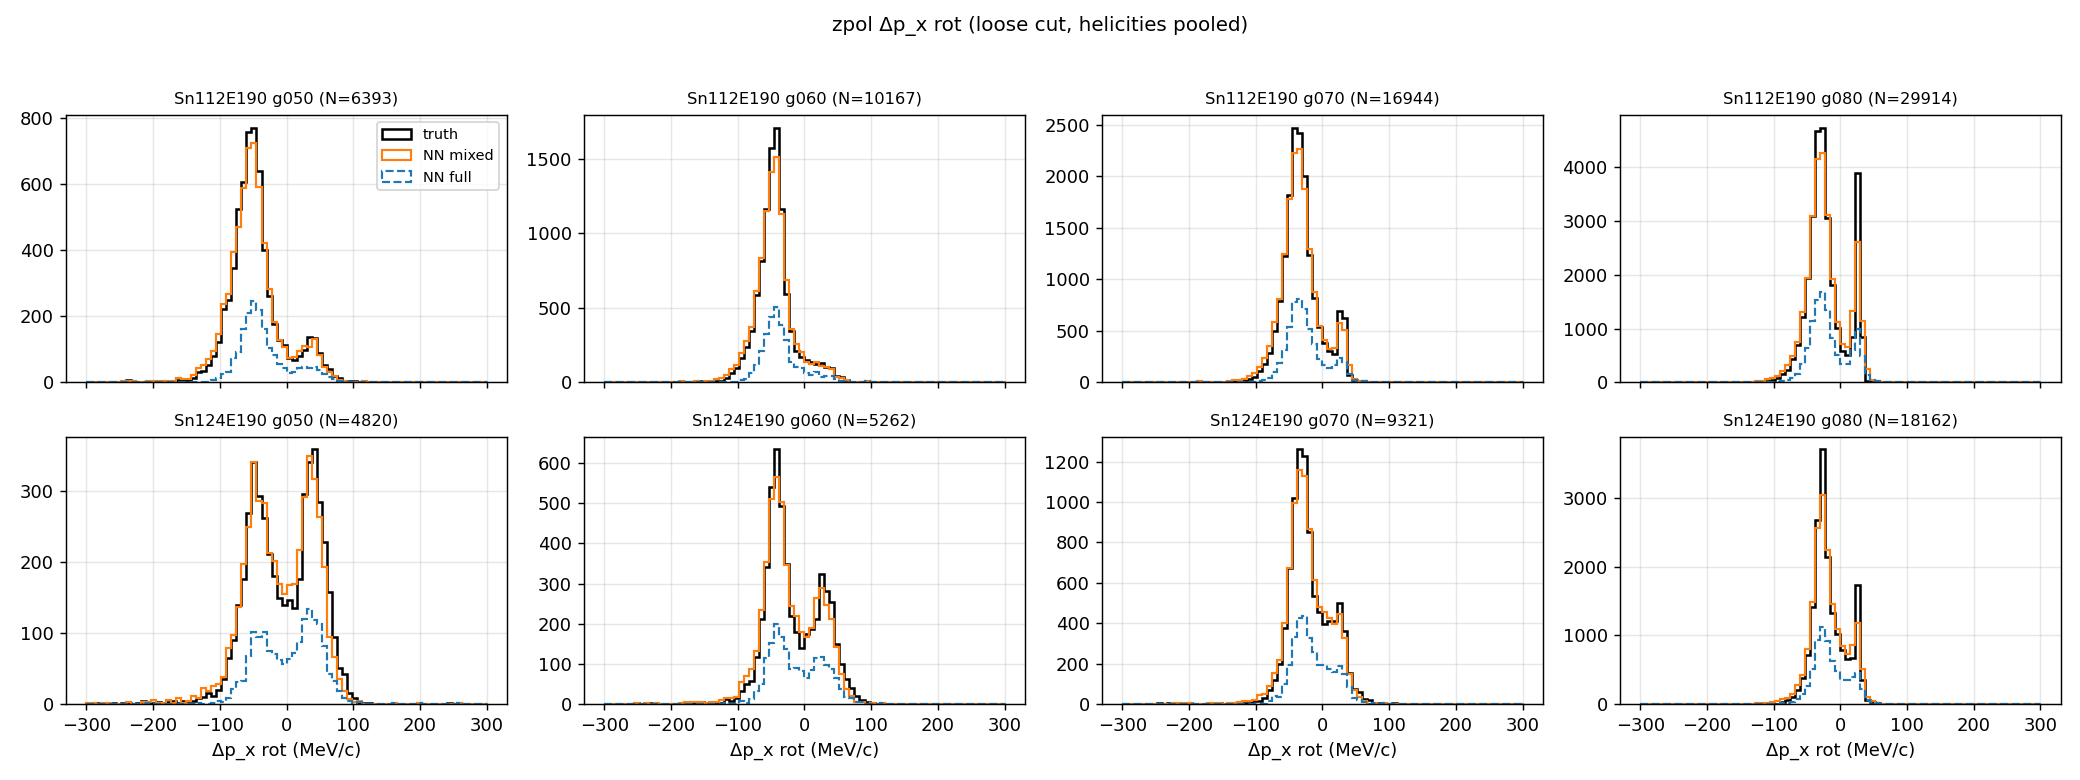
\includegraphics[width=0.85\textwidth]{figures/nn_breakup_phys/px_diff_hist_zpol_loose.png}
\caption{zpol $\Delta p_x^\text{rot}$ distribution (loose cut).}
\end{figure}
\begin{figure}[H]
\centering
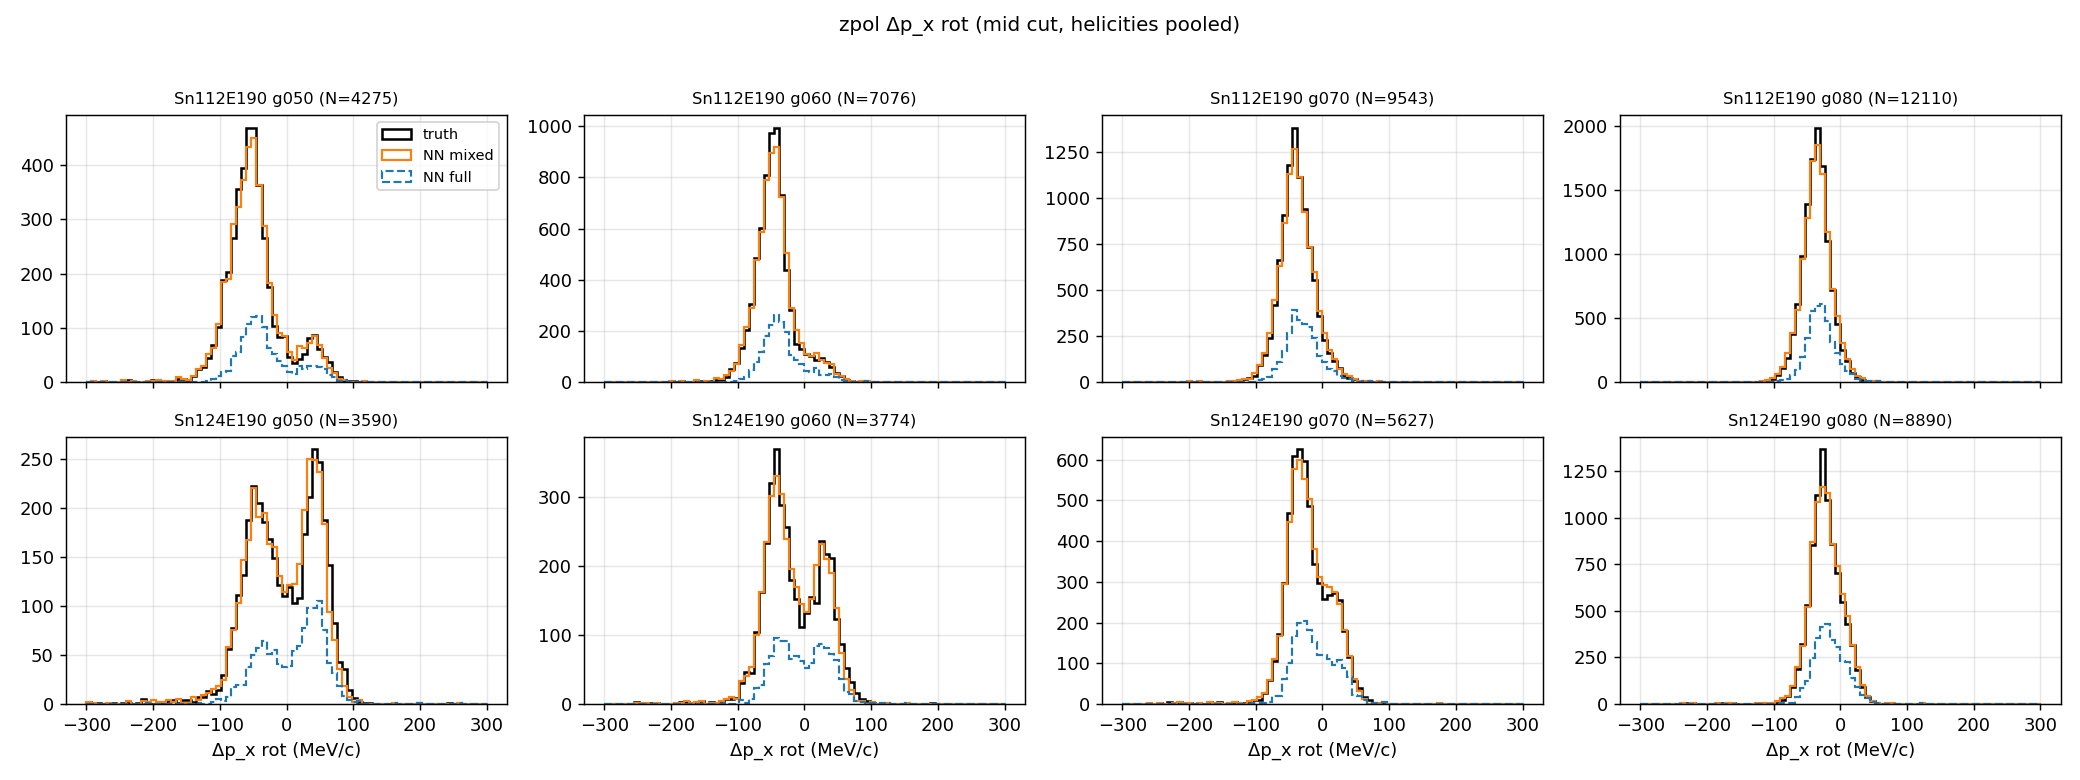
\includegraphics[width=0.85\textwidth]{figures/nn_breakup_phys/px_diff_hist_zpol_mid.png}
\caption{zpol $\Delta p_x^\text{rot}$ distribution (mid cut).}
\end{figure}
\begin{figure}[H]
\centering
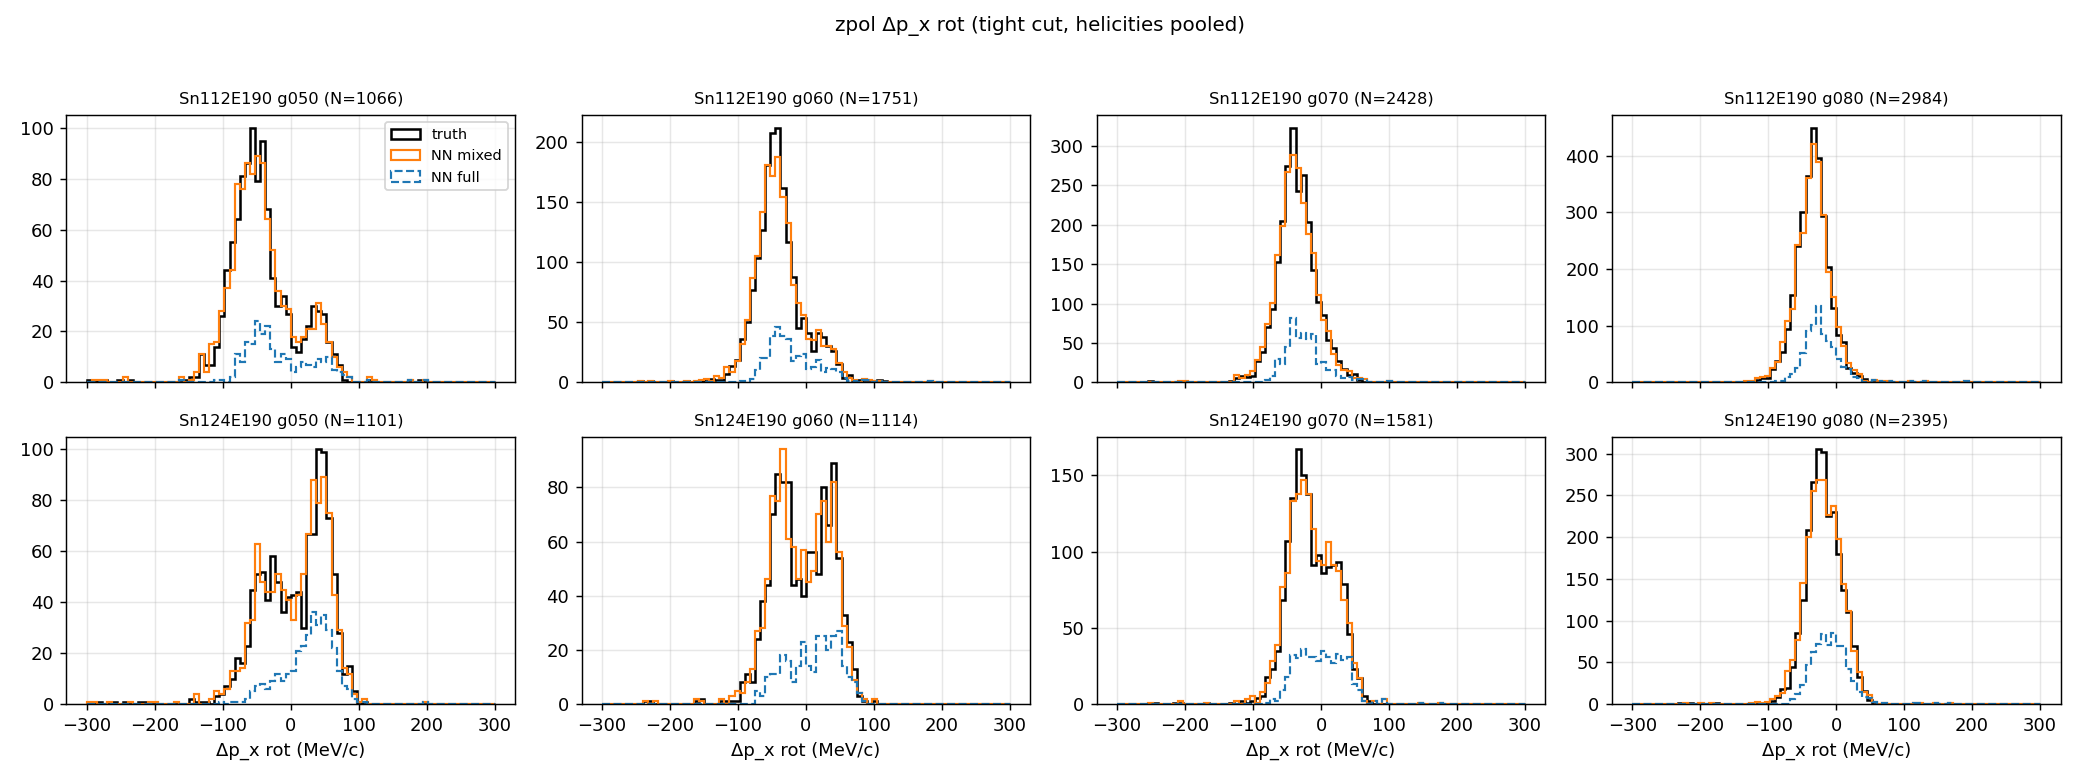
\includegraphics[width=0.85\textwidth]{figures/nn_breakup_phys/px_diff_hist_zpol_tight.png}
\caption{zpol $\Delta p_x^\text{rot}$ distribution (tight cut).}
\end{figure}

\subsection{6.4 zpol per-particle residuals}

\begin{figure}[H]
\centering
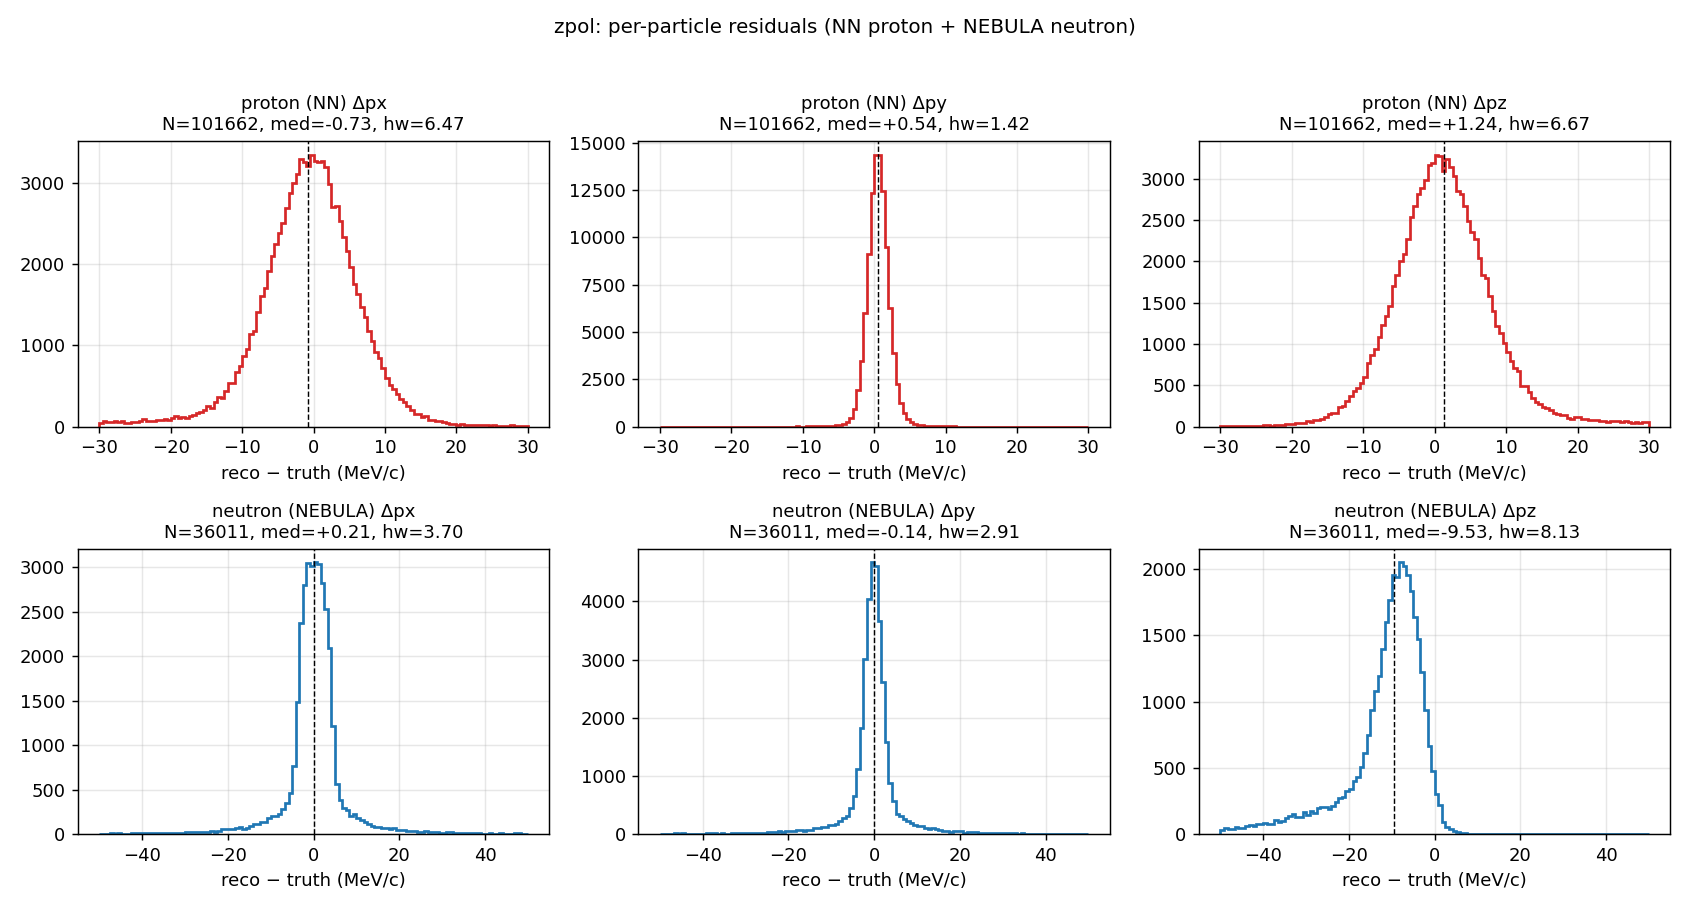
\includegraphics[width=\textwidth]{figures/nn_breakup_phys/residuals_per_particle_zpol.png}
\caption{zpol per-particle residuals. Top: NN proton; bottom: NEBULA neutron.}
\end{figure}

zpol training-domain coverage is 91.3\% (vs ypol 97.4\%); residuals are slightly wider than ypol but at the same order of magnitude --- not a meaningful perturbation to R.

\subsection{6.5 zpol reco vs truth 2D}
\begin{figure}[H]
\centering
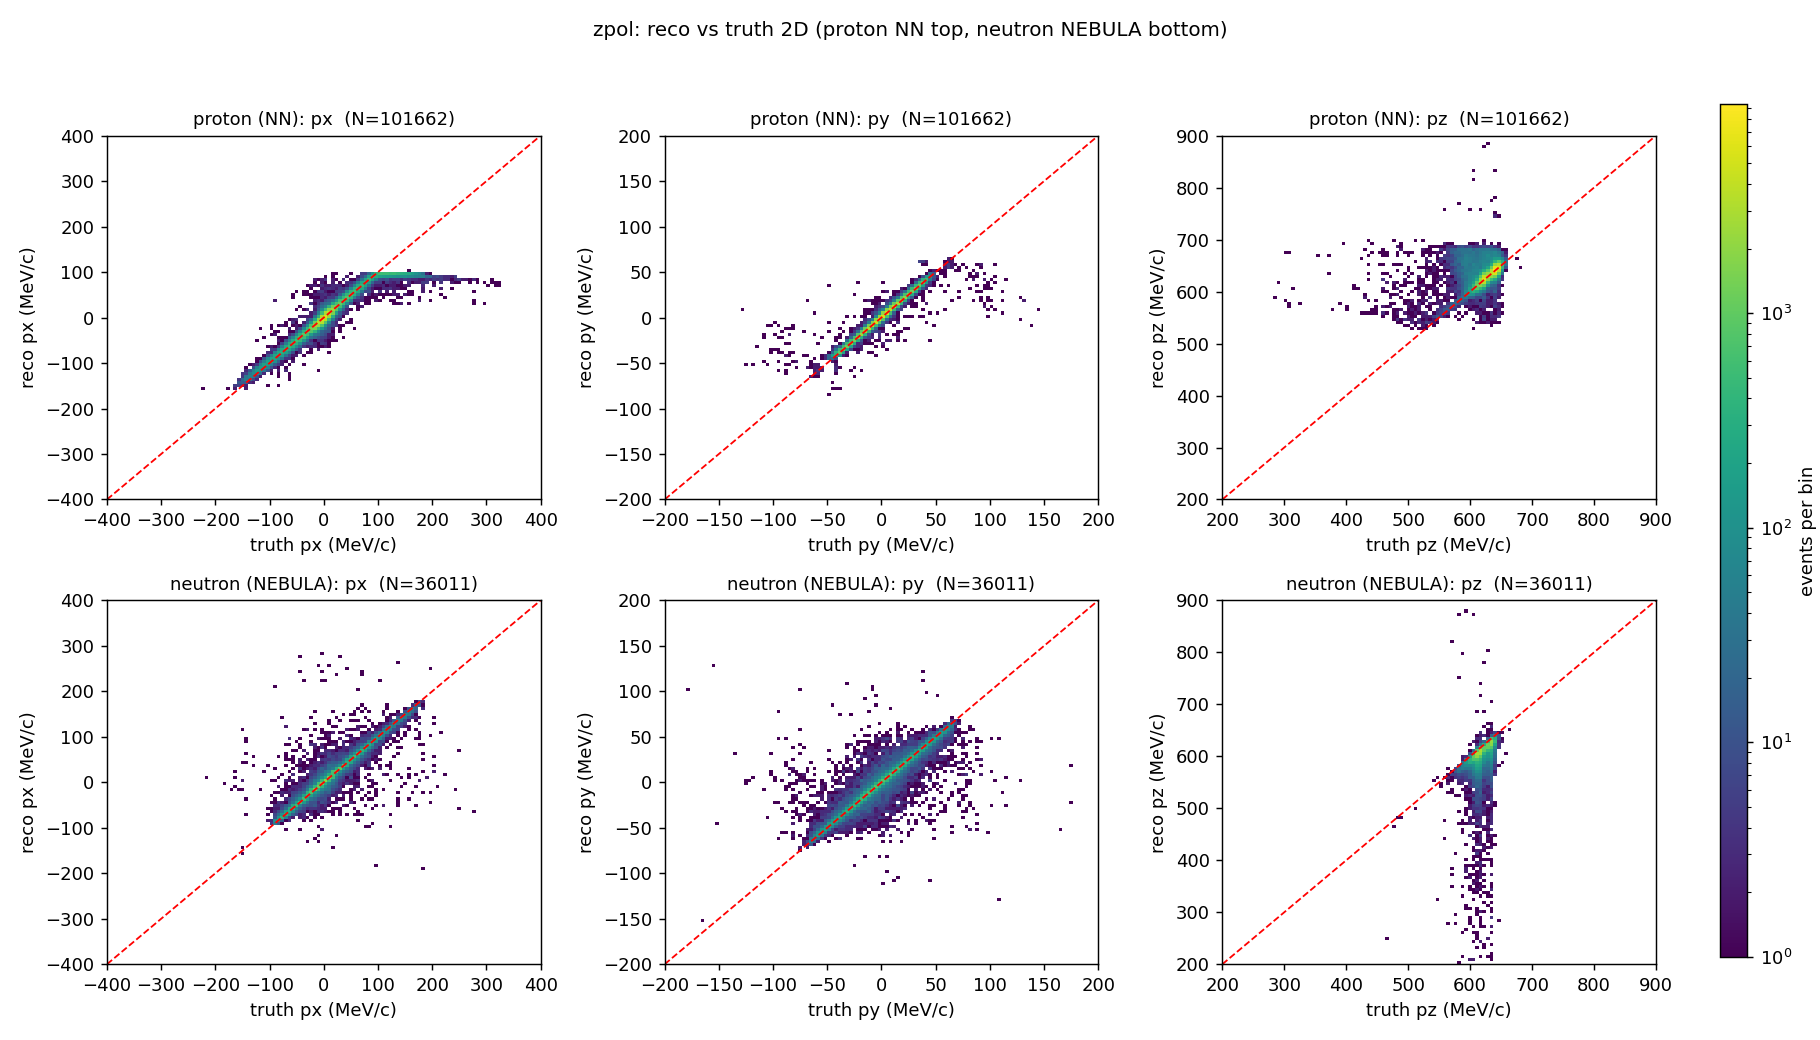
\includegraphics[width=\textwidth]{figures/nn_breakup_phys/reco_vs_truth_2d_zpol.png}
\caption{zpol reco vs truth 2D histograms. Top: NN proton; bottom: NEBULA neutron. Red dashed line $y=x$. All 6 panels share a common \texttt{LogNorm} color map; the right-side colorbar gives events per bin. Proton diagonal bends visibly outside the training domain ($|p_T| > 100$ MeV/$c$); neutron has the same NEBULA discrete-stepping structure as ypol.}
\end{figure}

\section{7. Conclusion \& next steps}

\begin{enumerate}[nosep]
    \item The production NN model runs stably as forward inference on breakup g4output, producing proton output for 100\% of cases.
    \item ypol Sn124 R signal is clean and decreases monotonically with gamma under all three cuts; zpol Sn124 signal is even stronger, with larger R range.
    \item NN B mixed vs A truth agrees to $<3\%$ on ypol and $<11\%$ on zpol; the latter is attributed to small statistics + neutron-fallback dependence and will be verified in the RK comparison.
    \item NN proton residual $\sigma$ on breakup matches elastic; training-domain coverage is 97\% (ypol) / 91\% (zpol), no significant extrapolation.
\end{enumerate}

\textbf{Follow-up reports}:
\begin{itemize}[nosep]
    \item \textbf{Next}: same spana03 g4output, RK reconstruction (after running on spana03), as a standalone report \texttt{rk\_breakup\_phys\_<date>\_zh.tex}.
    \item \textbf{After that}: \texttt{nn\_vs\_rk\_breakup\_phys\_<date>\_zh.tex}, head-to-head, focusing on (a) whether NN is significantly worse than RK in the large-$p_T$ extrapolation slice, and (b) whether the R deviation between the two methods is driven by a common NEBULA systematic.
\end{itemize}

\section*{Artifacts}
\begin{itemize}[nosep]
    \item rsync script: \texttt{scripts/analysis/nn\_breakup\_phys/00\_rsync\_from\_spana03.sh}
    \item NN reco driver: \texttt{scripts/analysis/nn\_breakup\_phys/01\_run\_nn\_reco.sh}
    \item Extraction macro: \texttt{scripts/analysis/nn\_breakup\_phys/02\_extract\_observables.C}
    \item Extraction driver: \texttt{scripts/analysis/nn\_breakup\_phys/run\_extract\_all.sh}
    \item R / $\Delta p_x$ analysis: \texttt{scripts/analysis/nn\_breakup\_phys/03\_analyze\_r\_breakup.py}
    \item Plotting: \texttt{scripts/analysis/nn\_breakup\_phys/04\_make\_figures.py}
    \item NN reco ROOT output: \texttt{data/reconstruction/breakup\_nn\_20260503/\{y\_pol,z\_pol\}/}
    \item Intermediate CSV: \texttt{build/test\_output/nn\_breakup\_phys\_20260503/csv/\{ypol,zpol\}/}
    \item R table / pass rates / joined df: \texttt{build/test\_output/nn\_breakup\_phys\_20260503/summary/\{ypol,zpol\}/}
\end{itemize}

\end{document}
